\section{Einführung}
\subsection{Unterschied Java vs C++}
Der Hauptunterschied zwischen Java und C++ ist, dass Java eine Interpretierte Sprache dh die Programmiersprache (bzw. der Bytecode) wird in einer Virtuellen Maschine ausgeführt namens JVM. 
Bei C++ werden die Instruktionen direkt von der CPU ausgeführt und es gibt keine Zwischensprache. Das bedeutet auch, dass C++ zwar schneller, aber dafür weniger portierbar ist.

Die Java-Laufzeit-Architektur ist folgendermassen\\
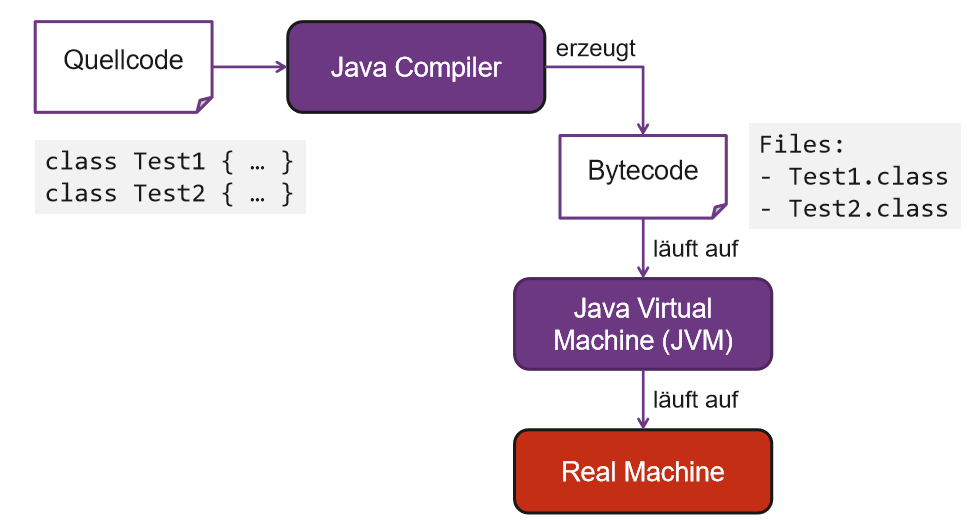
\includegraphics[width=\columnwidth]{Images/laufzeit_architektur}

\subsection{Datentypen}
Im Gegensatz zu c++ sind die Wertebereiche auf allen Platform gleich und es gibt keine unsigned Typen
\begin{center}
	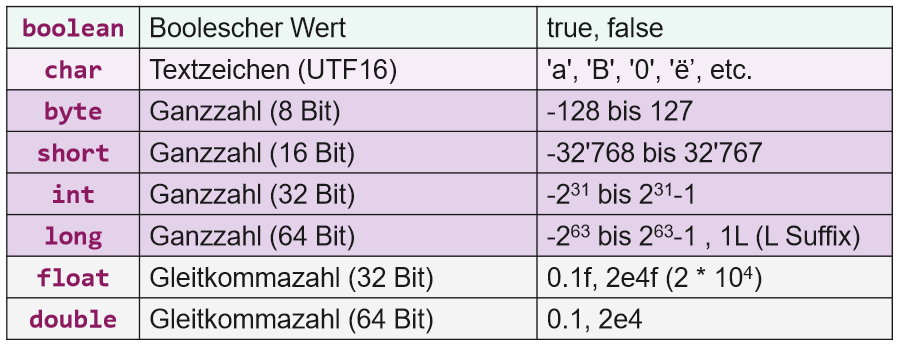
\includegraphics[width=\columnwidth,keepaspectratio=true]{Images/datentypen}
\end{center}

\subsection{Typumwandlung}
\begin{center}
	\begin{minipage}{0.1\textwidth}
		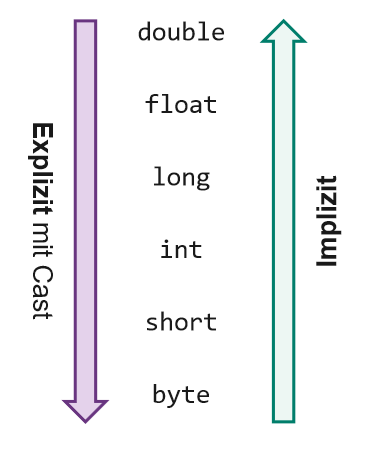
\includegraphics[width=\columnwidth,keepaspectratio=true]{Images/typumwandling}
	\end{minipage}%%% to prevent a space
	\begin{minipage}{0.35\textwidth}
		Die Typen werden in Java implizit umgewandelt, solange kein Datenverlust besteht. Sobald ein Datenverlust möglich ist, muss ein expliziter Cast verwendet werden.
	\end{minipage}
\end{center}

\noindent\textbf{Achtung} Wenn kein Literal angegeben ist, sind Zahlen standardmässig \textit{int}. Was bei Divisionen zu Fehlern führt, da Nachkommastellen Abgeschnitten werden $5 / 3 = 1$.

\subsection{Referenzsystem}
Variablen oder Parameter können via \underline{Call by Value} (Aufrufer sieht keine Änderung am Parameter - Kopie wird übergeben) oder \underline{Call by Reference} (Aufrufer sieht Änderungen an Parameter) aufgerufen bzw übergeben werden.\\

\noindent\textbf{Datentypen einordnung}\\
\begin{center}
	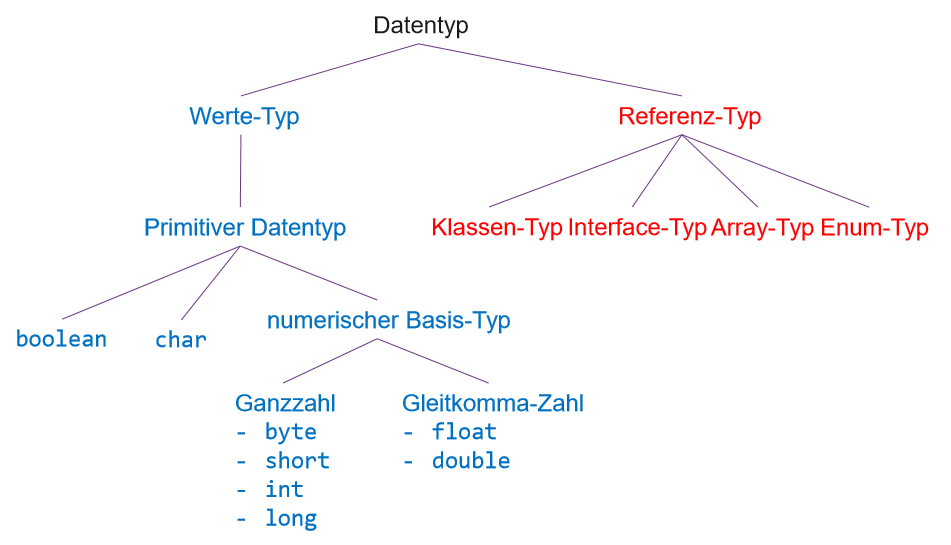
\includegraphics[width=0.7\columnwidth]{Images/datentypen_einordnung}
\end{center}
\begin{lstlisting}
Point a = new Point();
a.x = 0;
a.y = 1;

Point b = a;
b.x = 2;
b.y = 3;

System.out.println(a.x + " | " + a.y);
\end{lstlisting}
Die Ausgabe erzeugt "2 $|$ 3", da die Änderung für $a$ und $b$ gültig sind.


\noindent\textbf{Wichtig:} Wenn integer als Referenz benötigt werden, sollen Wrapper-Typen eingesetzt werden.
\begin{center}
	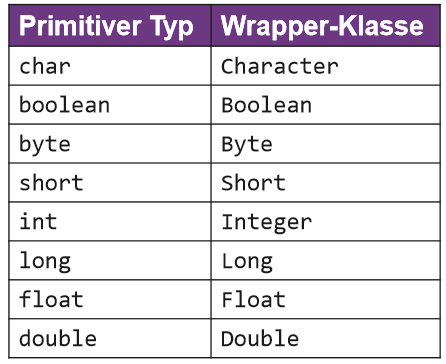
\includegraphics[width=0.4\columnwidth]{Images/wrapper}
\end{center}
\begin{lstlisting}
	// Boxing, oder auch: Integer.valueOf(123)
	Integer wrapper = 123;
	
	// Unboxing, oder auch: wrapper.intValue(), NullPointerException wenn wrapper == null
	int value = wrapper;
\end{lstlisting}
